\begin{figure}[h] % PBS and 20g/l solution
    \begin{minipage}{0.48\textwidth}
        \centering
        \begin{tikzpicture}[scale=0.85]
            \begin{semilogxaxis}[
                title={PBS solution}, xlabel=Frequency $(\si{\hertz})$, ylabel=Amplitude $(\si{\milli\volt})$, ymin=0, ymax=130, axis x line = bottom, axis y line=left,
            ]
                \addplot[] table{PBS.dat};
            \end{semilogxaxis}
        \end{tikzpicture}
    \end{minipage}
    \begin{minipage}{0.48\textwidth}
        \centering
        \begin{tikzpicture}[scale=0.85]
            \begin{semilogxaxis}[
                title={Yeast 20g/L solution}, xlabel=Frequency $(\si{\hertz})$, ylabel=Amplitude $(\si{\milli\volt})$,
                ymin=0, ymax=130, axis x line = bottom, axis y line=left,
            ]
            \addplot[] table{20gLGainOf100.dat};
            \end{semilogxaxis}
        \end{tikzpicture}
    \end{minipage}
    \caption{Amplitude based on frequency. Note the dip at \SI{50}{\hertz} due to the filter.}
    \label{gr:PBSand20gl}
    \end{figure}

Because there is no concern for cell disruption at the range of frequencies we are analysing (Yerworth, R., 2019 November 28), we can use Figure \ref{gr:PBSand20gl}, to find the maximum amplitude. PBS is around 3 kHz, and the yeast solution, 5 kHz. We expect to see equally as reasonable results by picking a simple average of the two, 4 kHz.

\begin{figure}[h!] %calibration curve
    \centering
    \begin{tikzpicture}
        \begin{semilogyaxis}[axis x line = bottom, axis y line=left,
            title={Calibration curve}, ylabel=Concentration \% , xlabel=Amplitude $(\si{\milli\volt})$,
            legend pos = north west,
            ]
            \addplot[only marks, forget plot] table{50gLGainOf100.dat};
            \addplot [
                dashed,
            ] table[ x={x},
                    y={ create col/linear regression = { y={y} } }
                ] {50gLGainOf100.dat};
            \addlegendentry{
                $\pgfmathprintnumber{\pgfplotstableregressiona} \cdot x\pgfmathprintnumber[print sign]{\pgfplotstableregressionb}$
            };
        \end{semilogyaxis}
    \end{tikzpicture}
    \caption{}
\end{figure}

\begin{figure}[h!] %24h run
    \centering
    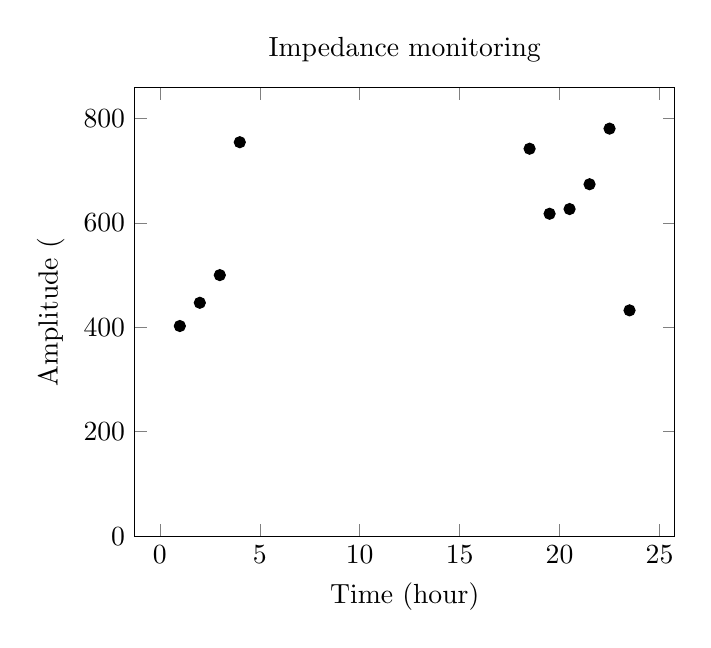
\begin{tikzpicture}
        \begin{axis}[xlabel=Time (hour), ymin=0, title={Impedance monitoring}, ylabel=Amplitude (\si{\milli\volt} ]
            \addplot[only marks] table{
                1	402.5
                2	447
                3	500
                4	754.5
                18.5	742
                19.5	617.5
                20.5	626.5
                21.5	674
                22.5	780.5
                23.5	432.5
            };
        \end{axis}
    \end{tikzpicture}
    \caption{Impedance monitoring during 24h run. The large jumps in numbers are due to accidental movement of the probes, invalidating the results.}
    \label{gr:24hImpedance}
\end{figure}
Originally it was expected that the impeller would not affect our results, but during the 24h run, we saw that the magnetism that drives the impeller had a very large effect on the numbers seen.
It is reasonable to take measurements while the impeller is in full use -- it is simply something to be account for in scaling up this project. 
Furthermore, as can be seen in Graph \ref{gr:24hImpedance}, the very first reading of the 24h run was \SI{400}{\milli\volt}, far greater than any result we observed during calibration.
We suspect a few issues in addition to those described in section \ref{sec:Impedance-Method}: Some deterioration of the tape that held the electrodes in place, as we produced the serial dilutions may have contributed to them floating in the liquid -- adding random error to our data.
This was exacerbated by having to stir the solutions by agitating the cup, further displacing the electrodes.

The 24 h setup was made ex novo, with the stirring and heating built in, and upon arrival there was a probe completely dislodged -- possibly it was bumped against while it was set up. No corrections were allowed, so adjusting the values to be in line with our calibration curve was not a possibility; and neither could we see through the dark liquid to adjust orientation. During the run, our magnetic stirrer would loosen out of its socket every few minutes, and in attempting to fix it, amplitude values ranged anywhere from \SI{200}{\milli\volt} to \SI{800}{\milli\volt}, completely hindering our ability to somehow normalise the data and compare to our calibration curve.

\paragraph{important comments on results, relate to theory and knowledge}